\documentclass[]{ceurart}
\input{macros}

% syntax highlighting for Pharo in code blocks
\include{./smalltalkEnv}

\begin{document}

%%
%% Rights management information.
%% CC-BY is default license.
\copyrightyear{2022}
\copyrightclause{Copyright for this paper by its authors.
  Use permitted under Creative Commons License Attribution 4.0
  International (CC BY 4.0).}

%%
%% This command is for the conference information
\conference{IWST'22: International Conference of Smalltalk Technologies,
August 24--26, 2022, Novy Sad, Serbia}

%%
%% The "title" command
\title{How Fast is AI in Pharo?\\Benchmarking Linear Regression}

%%
%% The "author" command and its associated commands are used to define
%% the authors and their affiliations.
\author[1,2]{Oleksandr Zaitsev}[%
orcid=0000-0003-0267-2874,
email=oleksandr.zaitsev@inria.fr,
]
\cormark[1]
\fnmark[1]

\author[2]{Sebastian Jordan-Montaño}[%
orcid=0000-0002-7726-8377,
email=sebastian.jordan@inria.fr,
]
\cormark[1]
\fnmark[1]

\author[2]{Stéphane Ducasse}[%
orcid=0000-0001-6070-6599,
email=stephane.ducasse@inria.fr,
]

\address[1]{Arolla,
25 Rue du Louvre, 75001 Paris, France}
\address[2]{Univ. Lille, Inria, CNRS, Centrale Lille, UMR 9189 CRIStAL,
Park Plaza, Parc scientifique de la Haute-Borne, 40 Av. Halley Bât A, 59650 Villeneuve-d'Ascq, France}

%% Footnotes
\cortext[1]{Corresponding author.}
\fntext[1]{These authors contributed equally.}


%%%%%%%%%%%%%%%%%%%%%%%

% %% Rights management information.  This information is sent to you
% %% when you complete the rights form.  These commands have SAMPLE
% %% values in them; it is your responsibility as an author to replace
% %% the commands and values with those provided to you when you
% %% complete the rights form.
% \setcopyright{acmcopyright}
% \copyrightyear{2022}
% \acmYear{2022}
% \acmDOI{XXXXXXX.XXXXXXX}

% %% These commands are for a PROCEEDINGS abstract or paper.
% \acmConference[IWST '22]{International Conference of Smalltalk Technologies}{August 24-26,
%   2022}{Novy Sad, Serbia}
% \acmPrice{15.00}
% \acmISBN{978-1-4503-XXXX-X/18/06}

% %Constants
% \newcommand{\numberOfSomething}{3}

% \begin{document}

% \title{How Fast is AI in Pharo?\\Benchmarking Linear Regression}
% \thanks{Both authors have equally contributed to this work.}

% \author{Oleksandr Zaitsev}
% \email{oleksandr.zaitsev@arolla.fr}
% \affiliation{%
%   \institution{Arolla, Inria, Univ. Lille, CNRS, Centrale Lille, UMR 9189 - CRIStAL}
%   \city{Lille}
%   \country{France}
% }

% \author{Sebastian Jordan Montaño}
% \email{sebastian.jordan@inria.fr}
% \affiliation{%
%   \institution{Inria, Univ. Lille, CNRS, Centrale Lille, UMR 9189 - CRIStAL}
%   \city{Lille}
%   \country{France}
% }

% \author{Stéphane Ducasse}
% \email{stephane.ducasse@inria.fr}
% \affiliation{%
%   \institution{Inria, Univ. Lille, CNRS, Centrale Lille, UMR 9189 - CRIStAL}
%   \city{Lille}
%   \country{France}
% }

% \renewcommand{\shortauthors}{Zaitsev et al.}

\begin{abstract}
As many other modern programming languages, Pharo spreads its applications into computationally demanding fields such as machine learning, big data, cryptocurrency, etc.
This raises a need for fast numerical computation libraries.
In this work, we propose to speed up the low-level computations by calling the routines from highly optimized external libraries, \eg LAPACK or BLAS through the foreign function interface (FFI).
As a proof of concept, we build a prototype implementation of linear regression based on the DGELSD routine of LAPACK.
Using three benchmark datasets of different sizes, we compare the execution time of our algorithm agains pure Pharo implementation and scikit-learn --- a popular Python library for machine learning.
We show that LAPACK\&Pharo is up to 2103 times faster than pure Pharo.
We also show that scikit-learn is 8-5 times faster than our prototype, depending on the size of the data.
Finally, we demonstrate that pure Pharo is up to 15 times faster than the equivalent implementation in pure Python. 
Those findings can lay the foundation for the future work in building fast numerical libraries for Pharo and further using them in higher-level libraries such as pharo-ai.
\end{abstract}

%%
%% Keywords. The author(s) should pick words that accurately describe
%% the work being presented. Separate the keywords with commas.
\begin{keywords}
  pharo \sep
  benchmarking \sep
  machine learning \sep
  foreign function interface \sep
  lapack \sep
  linear regression
\end{keywords}

%%
%% This command processes the author and affiliation and title
%% information and builds the first part of the formatted document.
\maketitle


%===========================================

\section{Introduction}
\label{sec:Introduction}

Pharo (\url{https://pharo.org/}) is an open-source dynamically-typed reflective, object-oriented programming language inspired by Smalltalk~\cite{Blac09a}.
Pharo community is growing and spreading its applications into various domains of modern computer science: big data~\cite{Marr20a,Marr22a}, machine learning~\cite{Berg20a},\footnote{\url{https://github.com/pharo-ai/wiki}} cryptocurrency,\footnote{\url{https://github.com/smartanvil/Fog}}\footnote{\url{https://github.com/oliveiraallex/Pharocks-Cryptobot}} internet of things (IoT)~\cite{Oliv21a}.
Those domains require fast numerical algorithms capable of working with large datasets.
Modern programming languages provide such libraries and use them as backend for more high-level ones such as scikit-learn\footnote{\url{https://scikit-learn.org/}}, a popular machine learning library.
Pharo also provides a library for numerical computations --- PolyMath.
However, as we will see in this paper, the current implementation of certain algorithms in Pharo is significantly slower than the ones provided by similar libraries in Python and R that delegate the low-lewel computations to the fast routines compiled in Fortran or C.

In this paper, we propose to speed up the numerical computations in Pharo by calling low-lewel routines from the highly optimized external libraries such as LAPACK or BLAS.
As a proof of concept, we propose a prototype implementation of the linear regression algorithm in Pharo based on the DGELSD routine of LAPACK.\footnote{All the code, the datasets, and the instructions on how to reproduce our experiment are available at \url{https://anonymous.4open.science/r/lapack-experiment-55FB}. }
We benchmark our algorithm against both an alternative implementation in pure Pharo and scikit-learn --- a widely used Python library for machine learning.

The Pharo \& LAPACK implementation is 1820 times faster than pure Pharo on a small-size dataset (200K rows) and 2103 times faster on a medium-size dataset (1M rows).
This serves as a proof of concept that the speed of numerical algorithms, and more specifically machine learning in Pharo can be significantly improved by calling highly optimized external libraries through FFI.
We also show that scikit-learn is still 8-5 times faster than our prototype implementation in Pharo (depending on the size of data), which might be caused by data preprocessing and other optimizations.
We propose to further explore this difference in future work.
Finally, we show that pure Pharo implementation of linear regression is about 5-15 times faster than the equivalent implementation in pure Python.
This can be explained by the just-in-time compilation performed by Pharo virtual machine.

The rest of this paper is structured in the following way.
In Section~\ref{sec:Problem}, we discuss the possibility of implementing a machine learning library in Pharo and the challenges associated with it.
In Section~\ref{sec:FFI}, we briefly explain the foreign function interface (FFI) and how it can be used to call C and Fortran routines from Pharo.
In Section~\ref{sec:LinearRegression}, we explain different implementations of the linear regression algorithm that we have selected for benchmarking.


%===========================================

\section{Can We Do Machine Learning in Pharo?}
\label{sec:Problem}

Modern machine learning is resource demanding.
It requires fast algorithms capable of processing large volumes of data.
Many algorithms in machine learning are based on matrix algebra and numerical optimization.
This raises the need for fast libraries that implement the basic algebraic operations such as matrix-vector multiplication and also highly optimized algebraic algorithms as singular value decomposition, Cholesky decomposition, eigenvector and eigenvalues calculation, etc. for different types of matrices, i.e., symmetric, orthogonal, hermitian, etc.

In Pharo, there is PolyMath --- a library for numerical computations and scientific computing.
With its 60 packages and 903 green tests\footnote{Measured at \url{https://github.com/PolyMathOrg/PolyMath} on June 1, 2022.} PolyMath provides a wide range of algorithms that cover various aspects of mathematics: differential equations, complex numbers, fuzzy algorithms, etc.
It also provides matrix algebra, statistical distributions, and numerical optimization methods that can be particularly useful for machine learning.
That being said, some algorithms that are implemented in PolyMath are very slow, compared to the similar numerical libraries in other languages.
For example, as we will see in Section~\ref{sec:Results}, the linear regression implementation that is based on the singular value decomposition (SVD) provided by PolyMath takes almost 5 hours to converge on a dataset with 5,000 rows and 5 columns.

There is also an ongoing effort in Pharo community to implement the tools for data science, machine learning, artificial intelligence, data mining, etc.\footnote{For the non-extensive list of different machine learning libraries and tools in Pharo, see \url{https://github.com/pharo-ai/awesome-pharo-ml}.}
One such library is \emph{pharo-ai} --- a collection of different machine learning algorithms implemented in Pharo: linear and logistic regression, support vector machines, K-means, naive bayes, etc.
It is inspired by \emph{scikit-learn}, a similar machine learning library in Python.
scikit-learn is a popular library that has many industrial applications.
Many of its algorithms are very fast because internally scikit-learn depends on a mathematical library \emph{scipy}, which in turn depends on \emph{LAPACK} --- an efficient low-level library implemented in Fortran that provides fast algorithms for linear algebra.

We propose to improve the speed of PolyMath and pharo-ai by calling LAPACK routines through foreign function interface --- a technique for calling external functions which is already implemented by Pharo (see Section~\ref{sec:FFI}).
In Figure~\ref{fig:libraries}, we show how LAPACK is used by scikit-learn in Python and propose a way how it could be used by pharo-ai library.
In this scheme, PolyMath implements various high-level mathematical algorithms by delegating low-level algebraic operations to LAPACK.
Then pharo-ai simply depends on PolyMath to implement fast machine learning algorithms.

As a proof of concept, in this paper we present a prototype implementation of linear regression in Pharo based on LAPACK.
We benchmark the training time of our model and show that it is almost 500 times faster than the pure Pharo implementation.

\begin{figure}
  \centering
  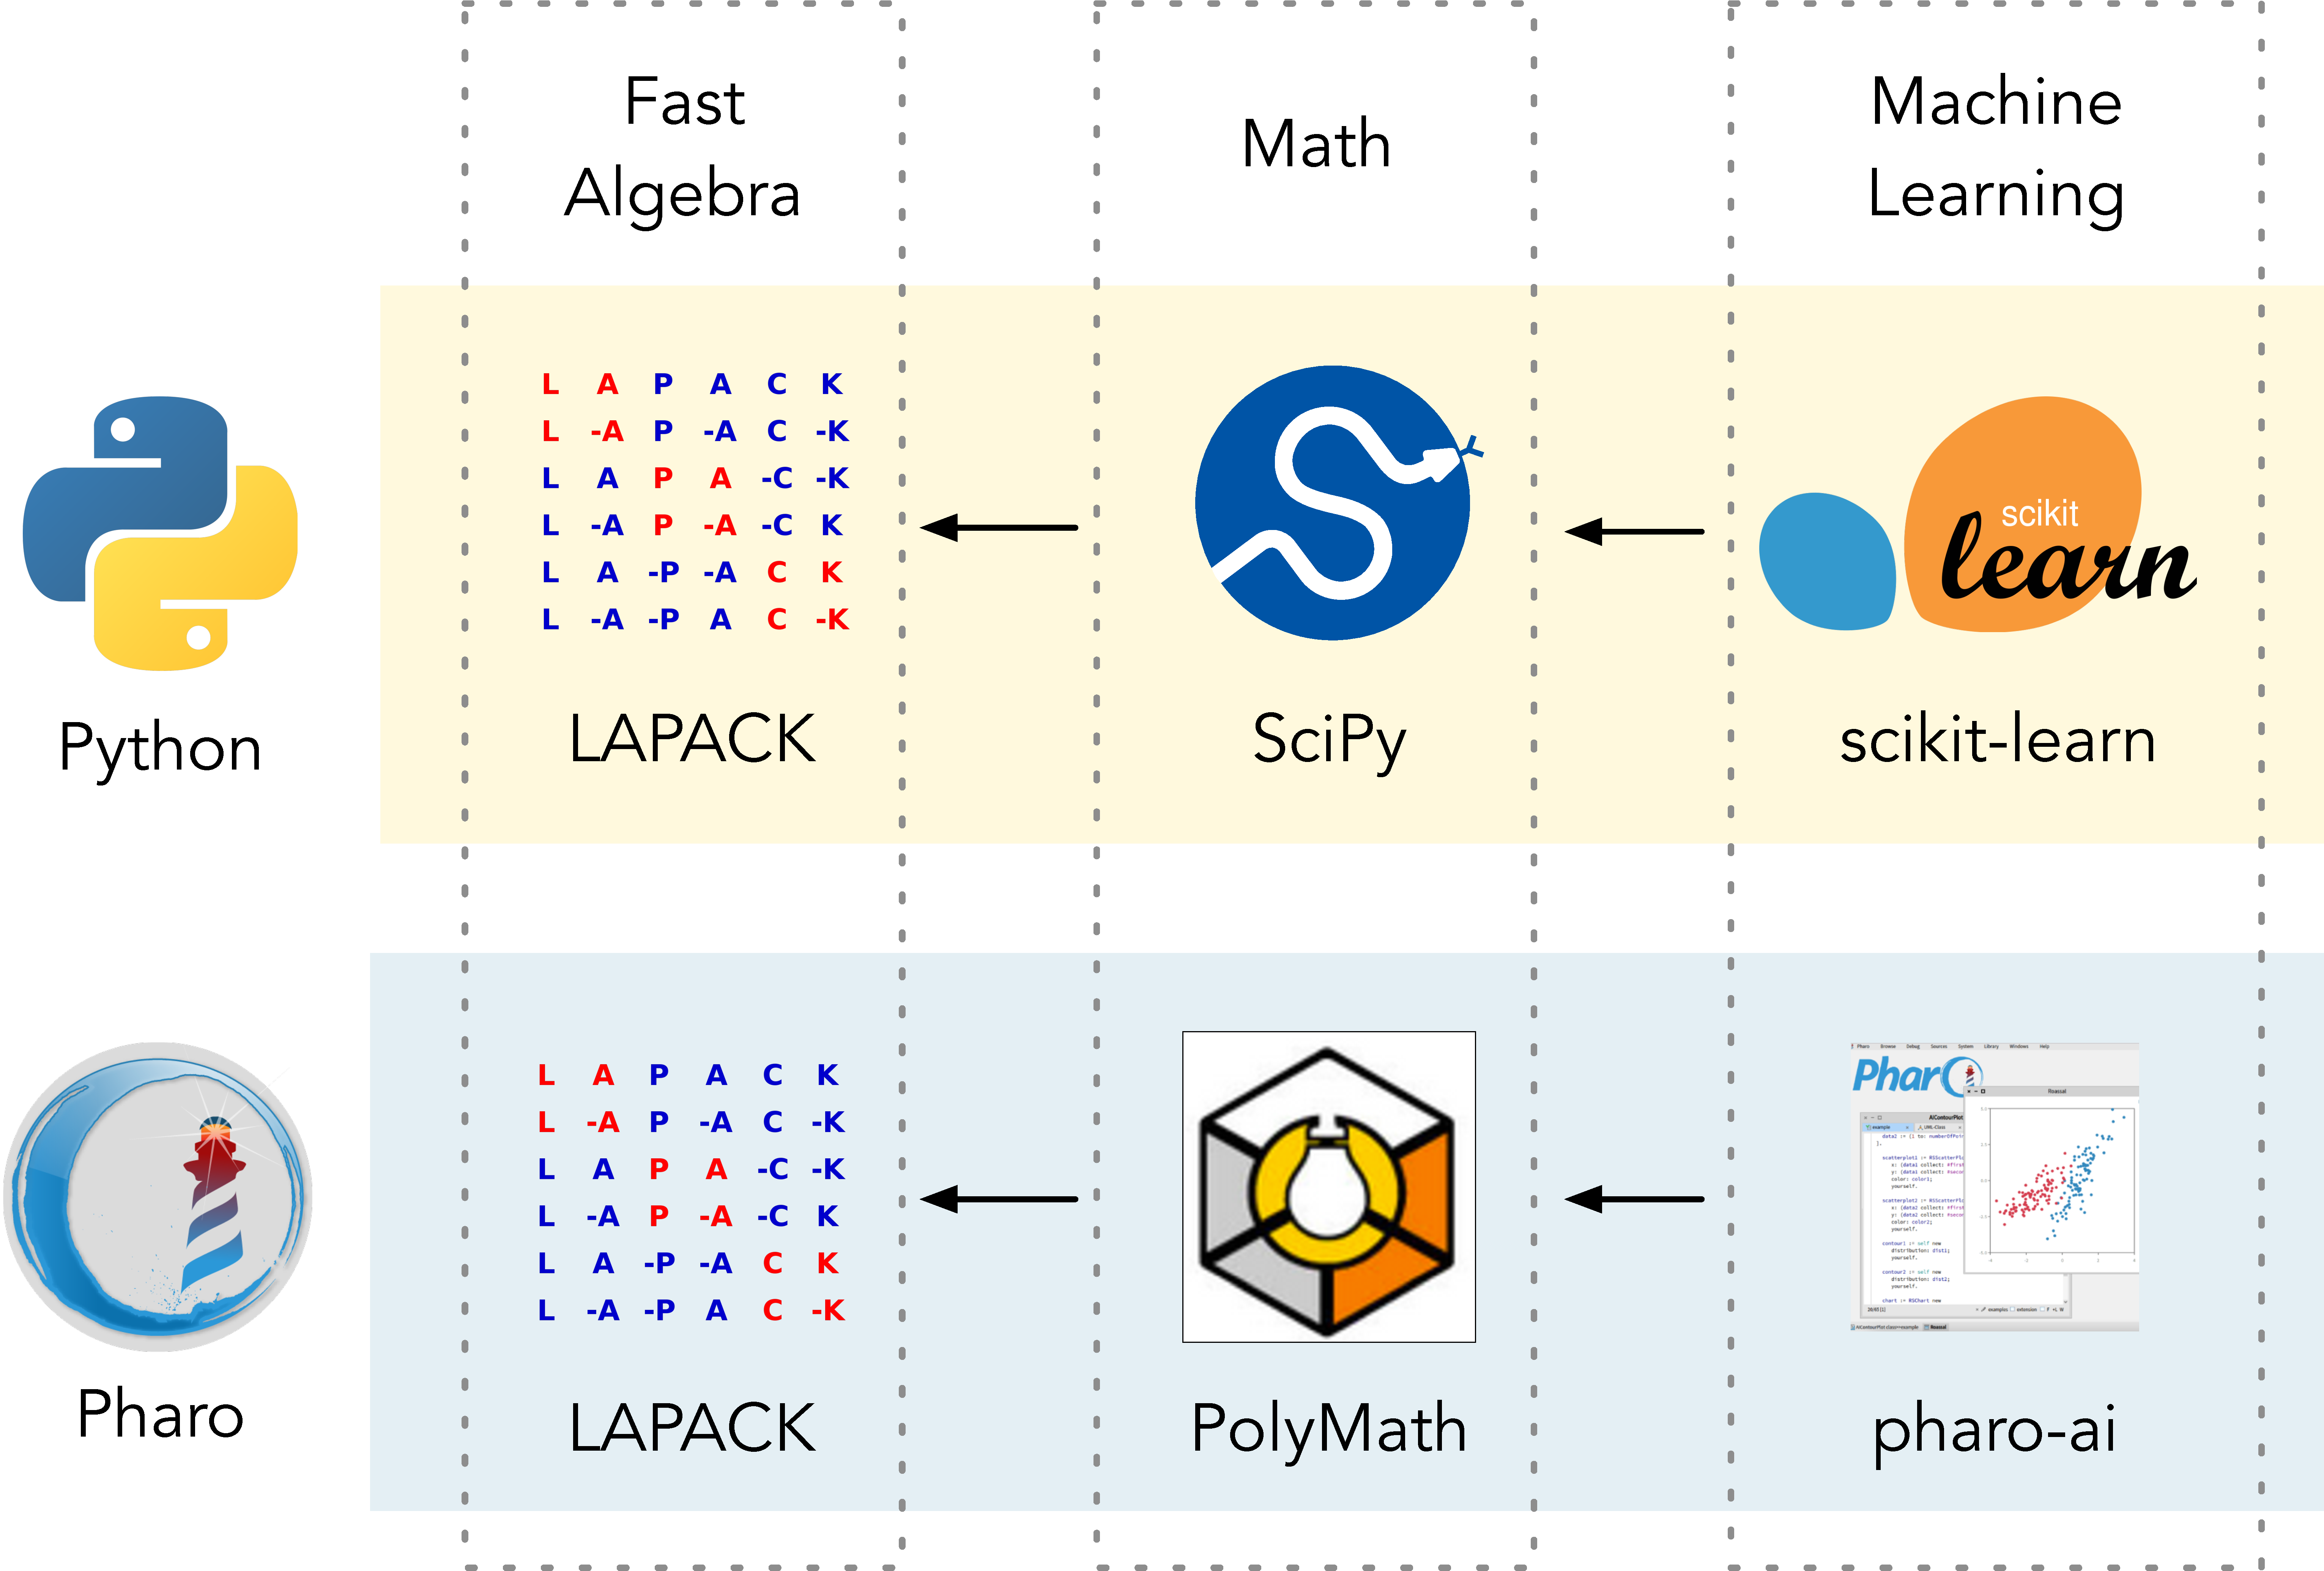
\includegraphics[width=.7\linewidth]{img/libraries}
  \caption{Machine learning libraries depend on mathematical libraries that in their turn depend on Lapack - a highly-optimized library providing fast algebraic operations.}
  \label{fig:libraries}
  \end{figure}


%===========================================

\section{Linear regression and How it is Implemented}
\label{sec:LinearRegression}

Linear Regression is a machine learning algorithms that models a relationship between the input matrix $X$ and the output vector $y$~\cite{Gero19a}.

\[ X = \begin{pmatrix}
x_{11} & \dots & x_{1n} \\
\vdots & \ddots & \vdots \\
x_{m1} & \dots & x_{mn}
\end{pmatrix};\quad
y = \begin{pmatrix}
y_{1} \\
\vdots\\
y_{m}
\end{pmatrix};\quad
\theta = \begin{pmatrix}
\theta_{0} \\
\vdots\\
\theta_{n}
\end{pmatrix}
\]

The task of linear regression is to find a set of parameters $\theta = (\theta_0, \dots, \theta_n)$ such that the predictions $\hat y_i = h_\theta(x_i)$ are as close as possible to the real output values $y_i$.
The function $h_\theta$ (also known as hypothesis function) is defined as:

\[ h_\theta(x_i) = \theta_0 + \theta_1 x_{i1} + \dots + \theta_n x_{in} \]

This is an optimization problem: we need to minimize the objective function that is often defined as \emph{mean squared error}:

\[ J(\theta) = \frac{1}{m} \sum_{i = 1}^m (y_i - h_\theta(X_{i:}))^2 \]

We have selected linear regression for benchmarking because: (1) it is one of the most well known and commonly used machine learning algorithms; (2) it can be solved by finding a minimum norm solution to the linear least squares problem --- an algorithm of linear algebra that is implemented in LAPACK.

\paragraph{Gradient Descent Solution}

Gradient descent is the iterative numerical optimization technique that is used by many machine learning algorithms, including linear regression.

It is based on the fact that derivative of the function in a given point is positive if the function is increasing and negative if it is decreasing.
This means that by subtracting the value of derivative $\frac{\partial}{\partial \theta_j} J(\theta)$, scaled by a parameter $\alpha$ (called the learning rate), from the current value of parameter $\theta_j$, we decrease the cost $J(\theta)$:

\[ \theta_j^{(new)} = \theta_j^{(old)} - \alpha \frac{\partial}{\partial \theta_j} J(\theta) \]

\paragraph{Least Squares Solution}

Alternatively, the problem of linear regression can be expressed in terms of linear least squares.
In this case, $X\theta = y$ is viewed as a system of linear equation where $\theta$ is the unknown.
Unless all points of the dataset lie on a straight line, this system has no solutions.
However, it is possible to find the closest approximation to the solution by solving the system $X\theta = \hat y$ where $\hat y$ is the orthogonal projection of $y$ onto the columnspace of $X$ (thus the distance between true output $y$ and predicted output $\hat y$ is the smallest).
This is the same as finding the optimal parameters $\hat \theta$ by minimizing the norm:

\[ \hat \theta = \text{argmin}\ \big|\big| y - X\theta \big|\big|_2 \]

In this work, we compare the following implementations of linear regression:

\begin{enumerate}
  \item Iterative gradient descent implementation in pure Pharo and pure Python.
  \item Least squares implementation in Pharo (our prototype) and Python (scikit-learn) that are both based on a routine from LAPACK library.
\end{enumerate}


%===========================================

\section{Foreign Function Interface in Pharo}
\label{sec:FFI}

As many modern programming languages, Pharo supports the \emph{Foreign Function Interface} (FFI) --- the mechanism that allows the call of routines from another programming language~\cite{Poli20z}.
One of the common uses is to speed up computations in interpreted or virtual machine languages by calling routines from natively compiled libraries (\eg \emph{*.dll} files on Windows or \emph{*.so} files on Linux and Mac).
Here is an example of calling a C function \ct{uint clock()} from Pharo using FFI:

\begin{lstlisting}[language=Smalltalk]
self
    ffiCall: #(uint clock())
    library: 'libc.so.6'.
\end{lstlisting}

The method \ct{ffiCall:library:} is understood by every object in Pharo.
It accepts two arguments which specify the shared library and the signature of a method that should be called.
The value returned by this method will be the same as the return value of the external function that is being called.

\paragraph{Calling LAPACK routine}

The Linear Algebra PACKage (LAPACK) is a Fortran library that provides routines for solving systems of simultaneous linear equations, least-squares solutions of linear systems of equations, eigenvalue problems, and singular value problems, matrix factorizations, etc.
In this work, we use one specific routine of LAPACK that computes the minimum-norm solution to a real linear least squares problem --- DGELSD.\footnote{\url{https://www.netlib.org/lapack/explore-html/d7/d3b/group__double_g_esolve_ga94bd4a63a6dacf523e25ff617719f752.html}}
It accepts as input matrix $X$ and vector $y$ and finds the solution vector $\hat \theta$ which minimizes the norm $||y - X\theta||_2$ (see Section~\ref{sec:LinearRegression}).


%===========================================

\section{Experiment Setup}
\label{sec:ExperimentSetup}

\paragraph{Research Questions} In our study, we answer the following research questions:

\begin{itemize}
% \renewcommand\labelitemi{---}
\item \emph{RQ.1 - Measuring LAPACK speedup.} How much time improvement can we achieve by calling LAPACK from Pharo?
\item \emph{RQ.2 - Comparing to scikit-learn.} How does Pharo \& LAPACK implementation compare to the one provided by scikit-learn?
\item \emph{RQ.3 - Comparing pure Pharo with Python.} How does pure Pharo implementation of linear regression compare to equivalent pure Python implementation?
\end{itemize}

\paragraph{Datasets for benchmarking}
We generated three datasets of different sizes using the \ct{make\_regression()} method of scikit-learn with a random linear regression model with a fixed seed.
The sizes of those datasets can be seen in Table~\ref{tab:Datasets}.
The number of columns was fixed at 20 and the number of rows was gradually increased.
We did this because the height (number of rows) and width (number of columns) of a dataset have different effect on the training time~\cite{Gero19a} and we did not want to mix them.

The first 19 columns represent the input matrix $X$.
They contain floating point numbers that are normally distributed around 0 with standard deviation 1.
The last column of each dataset represents the output vector $y$ generated by applying a non-biased linear regression model with gaussian noise.

\begin{table}[htbp]
\centering
\caption{Three datasets that we generated for this study}
\begin{tabular}{lrrr}
\hline
\textbf{Name} & \textbf{Columns} & \textbf{Rows} & \textbf{Size} \\
\hline
Small & 200,000 & 20 & 82 Mb \\
Medium & 1,000,000 & 20 & 411 Mb \\
Large & 5,000,000 & 20 & 2.06 Gb \\
\hline
\end{tabular}
\label{tab:Datasets}
\end{table}

\paragraph{Measuring the execution time}
In this study, we only measure that time that it takes to train the linear regression model as it is generally the most consuming part of the machine learning workflow.
In Pharo, we measure time using the \ct{timeToRun} method:

\begin{lstlisting}[language=Smalltalk]
time := [ "... some code..." ] timeToRun.
\end{lstlisting}

In Python, we use the \ct{time} library:

\begin{lstlisting}[language=Python]
import time

start_time = time.time()
# ... some code...
time = time.time() - start.time()
\end{lstlisting}


%===========================================

\section{Results}
\label{sec:Results}

In this section, we answer the research questions and discuss the results of our experiments.
The benchmarks were run in a MacBook Pro 2015 with a Intel i7 processor of 4 cores and 2.2G~Hz and 16~GB of RAM memory.
The operating system is Monterrey~v12.4.
To run the benchmarks, we closed all the applications that could be closed.
In addition, we disconnected the Internet and did not use the computer while experiment was in progress. The computer was plugged into the charger for the duration of the experiment.

\subsection*{RQ.1 - Measuring LAPACK speedup}

To answer the first research question, we measured the execution time of two implementations of linear regression on the three datasets that were discussed in Section~\ref{sec:ExperimentSetup}.
The first implementation was implemented in pure Pharo (no external libraries) and based on gradient descent.
The second implementation was based on least squares, implemented by calling the DGELSD LAPACK routine from Pharo.
As can be seen in Table~\ref{tab:LAPACKSpeedup}, the LAPACK implementation was 1820 times faster on small dataset and 2103 times faster on medium dataset.
We could not measure the execution time of pure Pharo implementation on large dataset because it was too long and we had to stop it after 5 hours.
The LAPACK implementation took about 15 seconds to converge on the same dataset. 

\begin{table}[htbp]
\centering
\caption{The speedup achieved by calling LAPACK routines fom Pharo.}
\begin{tabular}{l|cc|r}
\hline
\textbf{Dataset} & \textbf{Pharo} & \textbf{Pharo \& LAPACK} & \textbf{Diff} \\
\hline
Small & 00:19:39.090 & 00:00:00.648 & 1820$\times$ \\
Medium & 01:43:59.000 & 00:00:02.967 & 2103$\times$ \\
Large & $\infty$ & 00:00:15.676 & --- \\
\hline
\end{tabular}
\label{tab:LAPACKSpeedup}
\end{table}

\begin{cbox}
\textbf{Summary:} Calling LAPACK routines from Pharo can provide a significant speedup. The linear regression implemented with Pharo\&LAPACK is 462 times faster than the pure Pharo implementation when measured on small dataset and 284 times faster on medium dataset.
\end{cbox}

\subsection*{RQ.2 - Comparing to scikit-learn}

We compared the execution time of LAPACK-based implementation of linear regression in Pharo to the one provided by \ct{LinearRegression} class in scikit-learn, which is also based on the DGELSD routine of LAPACK.
As can be seen in Table~\ref{tab:CompareScikit}, scikit-learn is 8 times faster than our implementation on small dataset, 8 times faster on medium dataset, and 5 times faster on large dataset.
Considering that scikit-learn is well designed library with many industrial users and our implementation is a prototype, we hypothesize that this difference is due to various optimizations that are performed in scikit-learn.
For example, it uses a highly optimized data structure NumPy\footnote{\url{https://numpy.org/}}.
A further study is needed to explain this phenomenon.

\begin{table}[htbp]
\centering
\caption{Comparison with scikit-learn (both implementations use LAPACK).}
\begin{tabular}{l|cc|r}
\hline
\textbf{Dataset} & \textbf{Pharo \& LAPACK} & \textbf{scikit-learn} & \textbf{Diff} \\
\hline
Small & 00:00:00.648 & 00:00:00.079 & 8$\times$ \\
Medium & 00:00:02.967 & 00:00:00.790 & 8$\times$ \\
Large & 00:00:15.676 & 00:00:03.499 & 5$\times$ \\
\hline
\end{tabular}
\label{tab:CompareScikit}
\end{table}

\begin{cbox}
\textbf{Summary:} scikit-learn implementation is 8 times faster than our prototype implementation in Pharo. It is 5 times faster on a large dataset.
\end{cbox}

\subsection*{RQ.3 - Comparing pure Pharo with pure Python}

We also compare pure Pharo and pure Python implementations of linear regression based on gradient descent.
As can be seen in Table~\ref{tab:PharoPython}, Pharo is 5 times faster than Python on small dataset and 15 times faster on medium dataset.
We could not measure the execution time on large dataset, because in both cases it was too long and we had to stop the experiment.

\begin{table}[htbp]
\centering
\caption{Comparison between pure Pharo and pure Python}
\begin{tabular}{l|cc|r}
\hline
\textbf{Dataset} & \textbf{Pharo} & \textbf{Python} & \textbf{Diff} \\
\hline
Small & 00:19:39.090 & 01:39:54.275 & 5$\times$ \\
Medium & 01:43:59.000 & 08:25:00.000 & 15$\times$ \\
Large & $\infty$ & $\infty$ & --- \\
\hline
\end{tabular}
\label{tab:PharoPython}
\end{table}

\begin{cbox}
\textbf{Summary:} The implementation of gradient descent-based linear regression in pure Pharo (no external libraries) is about 5-15 times faster than the equivalent implementation in pure Python, depending on the size of the dataset.
\end{cbox}

%===========================================

\section{Threats to Validity}
\label{sec:Threats}

We consider the four types of validity threats that were presented by Wohlin~\etal~\cite{Wohl00a}: internal, external, construct, and conclusion validity.
Below, we discuss the threats to internal and external validity.
We did not find any threats to conclusion and construct validity.

\paragraph{Internal Validity}

\begin{itemize}
  \item The implementation of linear regression with LAPACK was based on least squares while the pure Pharo implementation was based on gradient descent. This poses a threat to internal validity because the time difference may be affected by the choice of algorithm.
  \item The implementation that we propose for Pharo is a prototype, while scikit-learn is the industry standard which contains many optimizations. We tried to study the source code of scikit-learn as much as possible, but this still constitutes a validity threat.
  \item Measuring the execution time is always prone to the noise introduced by different processes that are run on the computer. To reduce this noise, we have closed all unnecessary windows, disconnected the Internet, plugged the computer to the charger, and killed all processes that could be stopped.
\end{itemize}

\paragraph{External Validity}

\begin{itemize}
  \item In this work, we demonstrated how the training time of linear regression can be reduced using LAPACK. The same technique can be used for many other machine learning algorithms: logistic regression, neural networks, etc. Nonetheless, there are also algorithms that can not benefit from it because, unlike linear regression, they do not require heavy matrix-vector calculations. Some examples include k-means or k-nearest neighbours. Those algorithms can still be boosted with optimized C code called through FFI, but this requires a separate study.
\end{itemize}


%===========================================

\section{Related Work}
\label{sec:RelatedWork}

Over the years, Pharo has been successfully applied in various domains of scientific computing and numerical optimization.
Many of those applications use the algorithms provided by PolyMath~\cite{Bess16a} --- a library for scientific computing in Pharo.
Other applications depend on the algorithms of artificial intelligence and machine learning~\cite{Berg20a}.
Bergel~\etal~\cite{Berg18b} use neural networks and a visual environment to verify various properties related to the source code.
Cota~\etal~\cite{Cota20a} use genetic algorithms for automatic tests generation.
Pharo is also used for agent-based modeling by CORMAS (Common Pool Resources and Multi-Agent Systems) --- a platform dedicated to natural
and common-pool resources management~\cite{Bomm16a,Lepa12a}.
All those applications could benefit from speeding up numerical computations in Pharo.

In this work, we benchmark our prototype implementation of linear regression against scikit-learn --- a Python machine learning library that is widely used in both research and industry~\cite{Lang19a}.
Pedregosa~\etal~\cite{Pedr11a} report that scikit-learn outperforms other machine learning libraries in Python (MLP, PyBrain, pymvpa, MDP, and Shogun) in 4 out of 6 classical machine learning algorithms.

To the best of our knowledge, this is the first attempt to implement a fast numerical library in Pharo by calling an external library such as LAPACK.
It is also the first study that benchmarks the machine learning algorithms in Pharo.

%===========================================

\section{Conclusion}
\label{sec:Conclusion}

In this work we presented a proof of concept that demonstrates how numerical computations in Pharo can be boosted by calling the routines highly optimized external libraries through FFI.
We built a prototype implementation of linear regression algorithm in Pharo based on the DGELSD routine from LAPACK.
We measured the execution time on three benchmark datasets and compared it to the time that is needed to train the analogous models in scikit-learn and in pure Pharo.
We show that LAPACK-based implementation is up to 2103 times faster than pure Pharo but still 8-5 times slower than scikit-learn implementation, which also uses LAPACK underneeth.
We also show that pure Pharo implementation is up to 15 times faster than the equivalent model implemented in pure Python.
This interesting finding can be explained by just-in-time compilation that is performed by Pharo virtual machine.

\section{Acknowledgements}

We are grateful to Vincent Aranega and Guillermo Polito for their valuable advice and explanations of just-in-time compilation in Pharo.
Oleksandr Zaitsev also thanks Arolla\footnote{\url{https://arolla.fr}} software company for financing his work during this study.


\bibliography{rmod,others}
\end{document}